\documentclass[a4paper,11pt]{article}

\usepackage[utf8]{inputenc}
\title{ARC1 - TP 6}
\author{Aurélien Anne, Léo Noël-Baron \& Thierry Sampaio}
\date{13/11/2015}


\usepackage{a4wide}
\usepackage{textcomp}
\usepackage[utf8]{inputenc}
\usepackage[T1]{fontenc}
\usepackage[francais]{babel}

\usepackage{graphicx}
\usepackage[usenames,dvipsnames]{color}

\usepackage{hyperref} \urlstyle{sf}
\hypersetup{
  colorlinks=true,
  urlcolor=BlueViolet,
  citecolor=BlueViolet,
  linkcolor=BlueViolet,
}
\DeclareUrlCommand\email{\urlstyle{sf}}

\newenvironment{keywords}
  {\description\item[\bsc{Mots-clés}]~$\cdot$~ }
  {\enddescription}
\newenvironment{remarque}
  {\description\item[\bsc{Remarque} ---]\sl}
  {\enddescription}
\renewcommand{\thefootnote}{\arabic{footnote}}

\usepackage{listings}
\lstset{
  language=C,
  basicstyle=\ttfamily,
  keywordstyle=\color{OliveGreen},
  stringstyle=\color{Bittersweet},
  showstringspaces=false,
  commentstyle=\color{Gray},
  numbers=left,
  numberstyle=\ttfamily\color{Gray},
  frame=l,
  columns=fullflexible,
  rulecolor=\color{Gray},
  tabsize=4,
  extendedchars=true,
  literate=
	{É}{{\'E}}1 {è}{{\`e}}1 {à}{{\`a}}1 {È}{{\`E}}1 {À}{{\`A}}1 {ê}{{\^e}}1 {â}{{\^a}}1 {î}{{\^\i}}1 {ô}{{\^o}}1
	{Ê}{{\^E}}1 {Â}{{\^A}}1 {Î}{{\^I}}1 {Ô}{{\^O}}1 {Û}{{\^U}}1 {ë}{{\"e}}1 {ï}{{\"\i}}1 {ü}{{\"u}}1 {Ë}{{\"E}}1
	{Ï}{{\"I}}1 {Ü}{{\"U}}1 {û}{{\^u}}1 {ç}{{\c c}}1 {Ç}{{\c C}}1 {æ}{{\ae}}1 {Æ}{{\AE}}1 {œ}{{\oe}}1 {Œ}{{\OE}}1
	{é}{{\'e}}1,
}
\lstMakeShortInline{|}

\parskip=0.3\baselineskip
\sloppy

\makeatletter
  \let\runtitle\@title
  \let\runauthor\@author
\makeatother

\usepackage{fancyhdr}
\pagestyle{fancy}
\fancyhead{}
\lhead{\runtitle}
\rhead{\runauthor}
\setlength{\headheight}{13.6pt}

\usepackage{amssymb}
\usepackage{tikz}

\setlength{\parindent}{0em}
\usepackage{array}

\begin{document}

\maketitle

\subsection*{Protocole de demande-réponse entrelacée}

\begin{figure}[h]
\center
\begin{tikzpicture}[scale=0.17]
\tikzstyle{every node}+=[inner sep=0pt]
\draw [black] (25.7,-31.6) circle (3);
\draw (25.7,-31.6) node {$(0,\mbox{ }0)$};
\draw [black] (39.1,-21.5) circle (3);
\draw (39.1,-21.5) node {$(1,\mbox{ }0)$};
\draw [black] (52.7,-31.6) circle (3);
\draw (52.7,-31.6) node {$(0,\mbox{ }0)$};
\draw [black] (39.1,-38.6) circle (3);
\draw (39.1,-38.6) node {$(0,\mbox{ }1)$};
\draw [black] (28.1,-29.79) -- (36.7,-23.31);
\fill [black] (36.7,-23.31) -- (35.76,-23.39) -- (36.37,-24.19);
\draw (35.25,-27.05) node [below] {$Dem$};
\draw [black] (20.5,-35.4) -- (23.28,-33.37);
\fill [black] (23.28,-33.37) -- (22.34,-33.44) -- (22.93,-34.25);
\draw [black] (41.51,-23.29) -- (50.29,-29.81);
\fill [black] (50.29,-29.81) -- (49.95,-28.93) -- (49.35,-29.74);
\draw [black] (50.03,-32.97) -- (41.77,-37.23);
\fill [black] (41.77,-37.23) -- (42.71,-37.31) -- (42.25,-36.42);
\draw (44.11,-34.59) node [above] {$fin$};
\draw [black] (36.44,-37.21) -- (28.36,-32.99);
\fill [black] (28.36,-32.99) -- (28.84,-33.8) -- (29.3,-32.92);
\draw (29.22,-35.61) node [below] {$\overline{Dem}$};
\draw [black] (40.423,-41.28) arc (54:-234:2.25);
\draw (39.1,-45.85) node [below] {$Dem$};
\fill [black] (37.78,-41.28) -- (36.9,-41.63) -- (37.71,-42.22);
\draw [black] (22.734,-31.238) arc (290.77083:2.77083:2.25);
\draw (19.44,-26.58) node [left] {$\overline{Dem}$};
\fill [black] (24.18,-29.03) -- (24.37,-28.1) -- (23.43,-28.45);
\draw [black] (55.38,-30.277) arc (144:-144:2.25);
\draw (59.95,-31.6) node [right] {$\overline{fin}$};
\fill [black] (55.38,-32.92) -- (55.73,-33.8) -- (56.32,-32.99);
\end{tikzpicture}
\caption{Diagramme des états de DemRep}
\label{autodemrep}
\end{figure}

Le protocole demandé correspond à l'automate représenté en Figure \ref{autodemrep}, où chaque état est annoté des valeurs correspondantes des signaux $debut$ et $Rep$, l'état initial étant celui désigné par la flèche entrante. On peut alors réaliser cet automate par machine à jeton, avec un registre d'un bit par état, comme en Figure \ref{demrepjeton}, ou par codage dense.

\begin{figure}[h]
\center
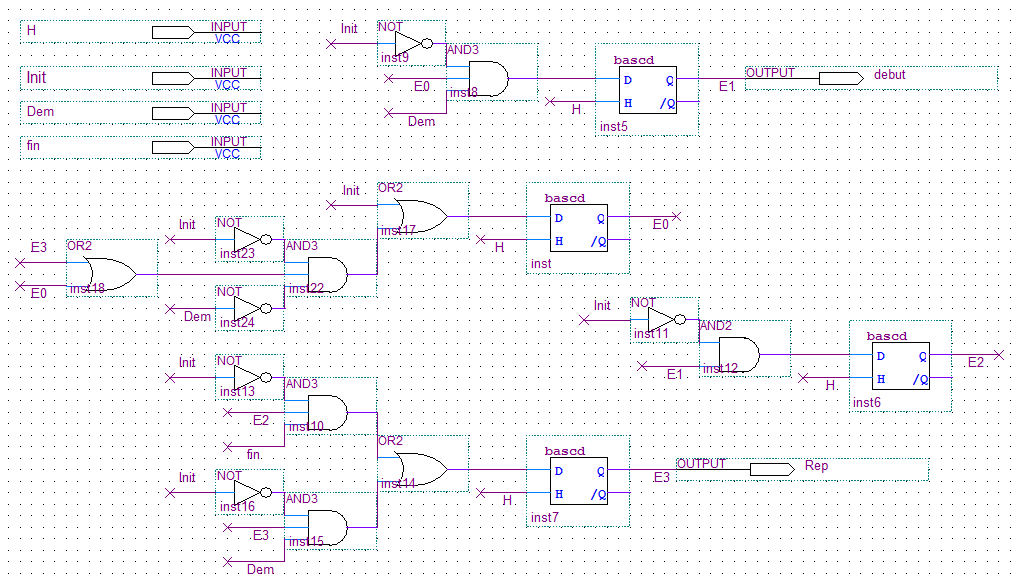
\includegraphics[scale=0.57]{DemRep.png}
\caption{Réalisation par machine à jeton}
\label{demrepjeton}
\end{figure}

Un codage dense envisageable est celui-ci, sur deux bits : 00 pour l'état 1, 01 pour 2, 10 pour 3 et 11 pour 4. En notant $q_1$ et $q_0$ les bits de codage, on a alors immédiatement $debut=\overline{q_1}q_0$ et $Rep=q_1q_0$, et une table des transitions permet d'obtenir les formules suivantes pour les deux registres : $q_1^+=\overline{q_1}q_0 + q_1\overline{q_0} + q_1Dem$ et $q_0^+ = \overline{q_1}\overline{q_0}Dem + q_1q_0Dem + q_1\overline{q_0}fin$. Ce codage donne le circuit présenté en Figure \ref{demrepdense}.

\begin{figure}[h]
\center
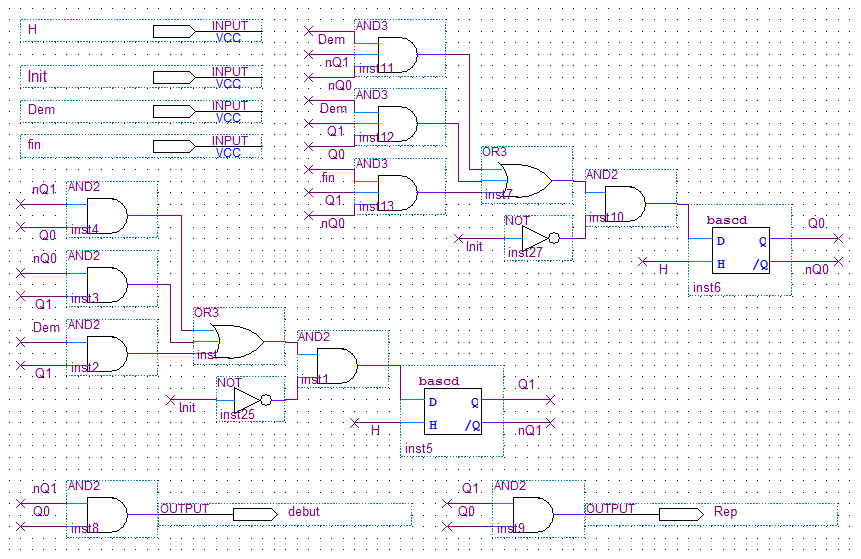
\includegraphics[scale=0.6]{DemRep2.png}
\caption{Réalisation par codage dense}
\label{demrepdense}
\end{figure}

Les deux circuits donnent des chronogrammes identiques en simulation, tel qu'en Figure \ref{simdemrep}.

\begin{figure}[h]
\center
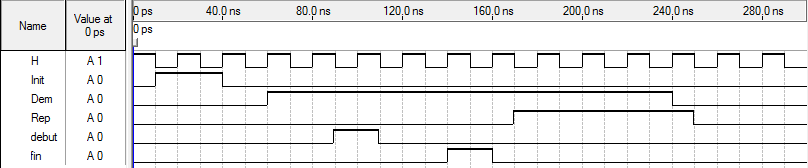
\includegraphics[scale=0.6]{simdemrep.png}
\caption{Simulation du protocole de demande-réponse}
\label{simdemrep}
\end{figure}


\subsection*{Générateur d'horloge}

\begin{figure}[h]
\center
\begin{tikzpicture}[scale=0.17]
\tikzstyle{every node}+=[inner sep=0pt]
\draw [black] (28.1,-31) circle (3);
\draw (28.1,-31) node {$0$};
\draw [black] (44.7,-27.5) circle (3);
\draw (44.7,-27.5) node {$1$};
\draw [black] (44.7,-41.1) circle (3);
\draw (44.7,-41.1) node {$2$};
\draw [black] (22.1,-31) -- (25.1,-31);
\fill [black] (25.1,-31) -- (24.3,-30.5) -- (24.3,-31.5);
\draw [black] (44.7,-30.5) -- (44.7,-38.1);
\fill [black] (44.7,-38.1) -- (45.2,-37.3) -- (44.2,-37.3);
\draw (44.2,-34.3) node [left] {$\overline{att}$};
\draw [black] (31.04,-30.38) -- (41.76,-28.12);
\fill [black] (41.76,-28.12) -- (40.88,-27.79) -- (41.08,-28.77);
\draw [black] (42.14,-39.54) -- (30.66,-32.56);
\fill [black] (30.66,-32.56) -- (31.09,-33.4) -- (31.61,-32.55);
\draw [black] (46.112,-24.866) arc (179.53768:-108.46232:2.25);
\draw (50.78,-22.2) node [right] {$att$};
\fill [black] (47.65,-27.02) -- (48.45,-27.53) -- (48.45,-26.53);
\end{tikzpicture}
\caption{Diagramme des états de GenHorl}
\label{autogenh}
\end{figure}

Le générateur d'horloge spécifié se comporte comme l'automate en Figure \ref{autogenh} ; initialement à l'état 0 (signal $HS = 1$), il passe immédiatement à l'état 1 puis y reste tant que la commande est activée (signal $HS = 0$), avant de passer à l'état 2 (signal $HS = 0$) qui revient à l'état initial. Un codage dense possible sur 2 bits est 10 pour l'état 0, 00 pour 1 et 01 pour 2 (afin d'avoir immédiatement $HS=q_1$ ; on prendra garde à l'état illicite 11). Les formules que doivent suivre les deux registres sont alors $q_1^+=\overline{q_1}q_0$ et $q_0^+=\overline{q_1}\cdot\overline{q_0}\cdot\overline{att}$, d'où le circuit présenté en Figure \ref{genhorl}.

\begin{figure}[h]
\center
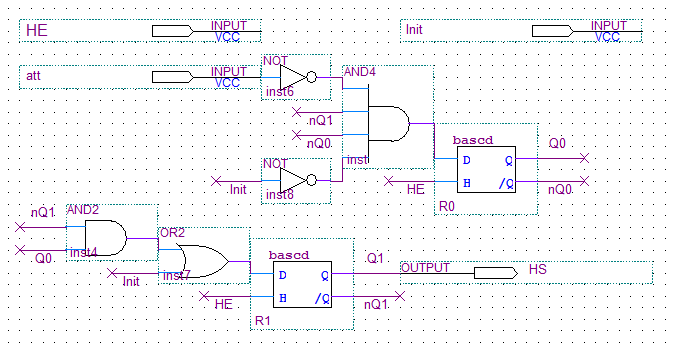
\includegraphics[scale=0.6]{GenHorl.png}\vspace*{1em}
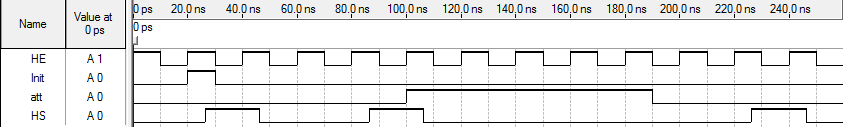
\includegraphics[scale=0.6]{sim.png}
\caption{Schéma et simulation du composant GenHorl}
\label{genhorl}
\end{figure}

\end{document}
